% strategy_report.tex -- Order Book Imbalance su BTC/USDT (G. Salvemini).
% Compilazione: pdflatex strategy_report.tex (due passaggi). Figure in figures/.
\documentclass[a4paper,11pt]{article}

\usepackage[utf8]{inputenc}
\usepackage[T1]{fontenc}
\usepackage[italian]{babel}
\usepackage{lmodern}
\usepackage{amsmath}
\usepackage{amssymb}
\usepackage{booktabs}
\usepackage{graphicx}
\usepackage{geometry}
\usepackage{float}
\usepackage{caption}
\usepackage{enumitem}
\usepackage{array}
\usepackage[hidelinks]{hyperref}

\geometry{margin=2.5cm}
\graphicspath{{figures/}}
\captionsetup{font=small,labelfont=bf}
\setlist{itemsep=2pt,topsep=4pt}

\newcommand{\OBI}{\mathrm{OBI}}
\newcommand{\WOBI}{\mathrm{WOBI}}
\newcommand{\EV}{\mathrm{EV}}
\newcommand{\bp}{\ensuremath{\,\mathrm{bp}}}
\newcommand{\usdt}{\ensuremath{\,\mathrm{USDT}}}
\newcommand{\code}[1]{\texttt{#1}}

\title{Order Book Imbalance su BTC/USDT:\\
dall'OBI al WOBI, e perché non basta\\[4pt]
\large Report di ricerca}
\author{Gianleonardo Salvemini\\[2pt]
\small Politecnico di Milano, Laurea Magistrale in Quantitative Finance}
\date{Settembre 2026}

\begin{document}

\maketitle

\begin{abstract}
\noindent
Lo squilibrio dei volumi nel limit order book (\emph{order book imbalance}) prevede il movimento
del mid-price di BTC/USDT nei secondi successivi? E si può guadagnare comprando e vendendo a
mercato quando il segnale è forte? Su 3.7 milioni di snapshot del book la risposta è sì alla
prima domanda e no alla seconda. Il segnale è reale e significativo anche out-of-sample, ma vale
tra 0.04 e 0.3\bp{} per lato, mentre una commissione taker su Binance costa tra 1.7 e 5\bp{}.
Usare dieci livelli del book invece del solo livello migliore rende il segnale più ordinato ma
non ne cambia l'ordine di grandezza. Ci sono arrivato dopo aver scoperto che la mia prima
versione, con un win rate sopra il 90\%, era piena di errori; la racconto nella
Sezione~\ref{sec:v1}.
\end{abstract}

\tableofcontents
\newpage

% ---------------------------------------------------------------------------
\section{Domanda e risposta in breve}
\label{sec:intro}

Il limit order book (LOB) raccoglie gli ordini limite in attesa, aggregati per livello di
prezzo: i \emph{bid} (chi vuole comprare) sotto il prezzo corrente, gli \emph{ask} (chi vuole
vendere) sopra. L'intuizione da cui sono partito è semplice: se al miglior bid c'è molto più
volume che al miglior ask, la coda dell'ask si esaurirà prima e il prossimo movimento del prezzo
sarà più probabilmente verso l'alto. So che è un'idea studiata nella letteratura sulla
microstruttura, anche se non ho ancora approfondito i lavori originali (ne elenco alcuni nella
Sezione~\ref{sec:letture}); mi sembrava un buon modo per lavorare per la prima volta su dati tick
reali.

Le domande erano due, e la risposta è diversa per ciascuna.

\begin{enumerate}[leftmargin=*]
  \item \textbf{Il segnale predice il prezzo? Sì.} Più il book è sbilanciato, più il mid si
        muove nella direzione prevista, anche sui dati che non ho usato per scegliere i
        parametri (t-stat fino a circa 57). È il grafico della Sezione~\ref{sec:ris-predice}.
  \item \textbf{Ci si guadagna comprando e vendendo a mercato? No.} Il guadagno medio per
        trade, prima delle commissioni, equivale a una commissione di 0.04--0.3\bp{} per lato.
        Su Binance un taker paga tra 1.7\bp{} (livello VIP più alto) e 5\bp{} (livello
        standard)\footnote{Tariffe dei futures USD\textsuperscript{\tiny S}-M di Binance: taker
        0.05\% al livello standard e 0.017\% al livello VIP più alto,
        \url{https://www.binance.com/en/fee/futureFee}.}: da 5 a 130 volte di più. Nessuna
        scelta di soglia, orizzonte o take-profit colma questa distanza
        (Sezione~\ref{sec:ris-nonpaga}).
\end{enumerate}

All'inizio consideravo la seconda domanda un dettaglio; il lavoro è stato in gran parte
scoprire che era quella principale. La conclusione che ne traggo è che l'imbalance può servire
a decidere \emph{come} quotare (market making), non \emph{se} attraversare lo spread; con questi
dati però non posso verificarlo in modo credibile (Sezione~\ref{sec:limiti}).

\paragraph{Come leggere il report.} Le Sezioni~\ref{sec:dati}--\ref{sec:esecuzione} spiegano
dati, segnale e regole del backtest; la Sezione~\ref{sec:risultati} contiene i risultati; la
Sezione~\ref{sec:v1} racconta la prima versione e gli errori che conteneva. In appendice ci sono
il motore di calcolo e i benchmark (Appendice~\ref{app:calcolo}), le tabelle complete
(Appendice~\ref{app:tabelle}) e l'elenco di tutte le assunzioni (Appendice~\ref{app:assunzioni}).

% ---------------------------------------------------------------------------
\section{Dati}
\label{sec:dati}

Uso il dataset Kaggle \emph{Bitcoin Limit Order Book (LOB) Data}~\cite{kaggle}: 3\,730\,870
snapshot del book del perpetual BTCUSDT di Binance dal 9 al 20 gennaio 2023 (circa 11 giorni),
uno ogni 250\,ms, con 10 livelli di prezzo per lato. I prezzi sono in USDT e i volumi in BTC
frazionari. Nel periodo BTC vale tra 17\,100 e 21\,700\usdt{}, quindi un punto base (bp) vale
circa 2\usdt{}.

Tre caratteristiche dei dati contano per tutto il resto (statistiche complete nella
Tabella~\ref{tab:data-summary} in appendice):
\begin{itemize}[leftmargin=*]
  \item \textbf{Lo spread è quasi sempre minimo}: pari a un tick (0.1\usdt{}) nel 99.2\% degli
        snapshot. Tutto ciò che il segnale può guadagnare si gioca su movimenti di pochi decimi
        di USDT.
  \item \textbf{Ci sono buchi nei dati}: 296 intervalli tra snapshot superiori a 500\,ms, il più
        lungo di 93\,s. Per questo misuro gli orizzonti in millisecondi e non in numero di
        snapshot, ed escludo i trade che attraversano un buco di oltre 2\,s.
  \item \textbf{Per il resto i dati sono puliti}: nessun book incrociato, nessun valore mancante,
        timestamp sempre crescenti. Li controllo con una funzione (\code{sanity\_check}) che
        conta i problemi invece di scartare righe in silenzio.
\end{itemize}

Divido i dati in ordine cronologico: il primo 70\% (fino al 17 gennaio) è
\emph{in-sample}, gli ultimi tre giorni circa sono \emph{out-of-sample}. Salvo indicazione
contraria i numeri che cito sono out-of-sample.

% ---------------------------------------------------------------------------
\section{Il segnale}
\label{sec:segnale}

Indico con $k$ lo snapshot (timestamp $t_k$ in ms) e con $i=0,\dots,9$ il livello, dove $0$ è
il miglior prezzo, detto anche \emph{touch}. $P^b_i, V^b_i$ sono prezzo e volume del bid,
$P^a_i, V^a_i$ quelli dell'ask. Il mid-price è $m = (P^b_0 + P^a_0)/2$ e lo spread
$s = P^a_0 - P^b_0$.

\paragraph{OBI (livello 1).} La misura più semplice di squilibrio usa solo il touch:
\begin{equation}
  \OBI = \frac{V^b_0 - V^a_0}{V^b_0 + V^a_0} \in [-1, 1].
  \label{eq:obi}
\end{equation}
Vale $+1$ se c'è volume solo sul bid, $-1$ se solo sull'ask.\footnote{Se la somma dei volumi è
zero l'OBI vale 0; se un volume è mancante (NaN) il segnale resta NaN, perché un dato corrotto
non deve sembrare un book bilanciato.} La regola di trading è altrettanto semplice: data una
soglia $\theta$ (di riferimento $0.6$) compro a mercato se $\OBI > \theta$, vendo se
$\OBI < -\theta$, e chiudo dopo un orizzonte fisso $H$.

\paragraph{WOBI (dieci livelli).} Il livello 1 descrive solo la coda esposta; i livelli più
profondi dicono quanta liquidità resta quando il touch si esaurisce. Il WOBI è lo stesso
rapporto calcolato sui volumi dei primi $D=10$ livelli, pesati con $w_i = e^{-\alpha i}$
($\alpha = 0.5$): il touch pesa 1 e ogni livello più profondo conta meno, perché gli ordini
lontani vengono eseguiti più di rado e cancellati più spesso.
\begin{equation}
  \WOBI = \frac{\sum_i w_i V^b_i - \sum_i w_i V^a_i}{\sum_i w_i V^b_i + \sum_i w_i V^a_i}.
  \label{eq:wobi}
\end{equation}

\paragraph{Micro-price ed edge.} La strategia WOBI usa anche un ``prezzo giusto'' che tiene
conto dei volumi:
\begin{equation}
  \mu = \frac{\sum_i w_i \left( V^b_i\, P^a_i + V^a_i\, P^b_i \right)}
             {\sum_i w_i \left( V^b_i + V^a_i \right)} .
  \label{eq:micro}
\end{equation}
La ponderazione è incrociata: molto volume sul bid sposta $\mu$ verso l'ask, cioè verso dove
il prezzo probabilmente andrà. L'\emph{edge} $e = \mu - m$ misura in USDT quanto il prezzo
giusto si discosta dal mid, ed è quindi confrontabile direttamente con spread e commissioni.

Un conto di due righe mi ha chiarito molto. Con un solo livello ($D=1$)
\begin{equation}
  \mu_1 - m = \frac{s}{2}\,\OBI ,
  \label{eq:micro1}
\end{equation}
cioè al livello 1 il micro-price è solo l'OBI riscalato per metà spread: con uno spread di un
tick, $|\mu_1 - m| \le 0.05\usdt{}$. Tutto ciò che il micro-price aggiunge viene dai livelli
profondi. Sul dataset $|e|$ ha mediana 0.05\usdt{} e 99-esimo percentile 0.37\usdt{}: il
segnale vive quasi tutto dentro un tick.

La mia formula per $\mu$, che accoppia il livello $i$ del bid con il livello $i$ dell'ask, è
un'euristica, da trattare come una feature da valutare e non come un modello. In letteratura
esiste una definizione di micro-price stimata dai dati, dovuta a Stoikov, che non ho ancora
studiato (Sezione~\ref{sec:letture}).

% ---------------------------------------------------------------------------
\section{Come simulo un trade}
\label{sec:esecuzione}

Entrambe le strategie passano per lo stesso motore di backtest (\code{src/lobimb/backtest.py}),
che segue regole fisse. Le ho scritte tutte perché nella prima versione erano proprio le regole
implicite a falsare i risultati (Sezione~\ref{sec:v1}).

\subsection{Le regole}

\begin{enumerate}[leftmargin=*]
  \item \textbf{Latenza.} Un segnale allo snapshot $k$ non si esegue subito: il fill avviene al
        primo snapshot $\ell$ almeno $L = 250$\,ms dopo, cioè di solito quello successivo.
  \item \textbf{Entrata da taker.} Compro all'ask, $p^{\mathrm{in}} = P^a_{\ell,0} + \sigma$,
        o vendo al bid, $p^{\mathrm{in}} = P^b_{\ell,0} - \sigma$, dove $\sigma$ è uno
        slippage per lato (0 nei risultati riportati).
  \item \textbf{Uscita.} Per l'OBI esco al primo snapshot almeno $H$ dopo il fill. Per il
        WOBI uso un \emph{bracket}: esco appena il prezzo a cui potrei chiudere ha guadagnato
        TP o perso SL rispetto a $p^{\mathrm{in}}$, e comunque dopo 2.5\,s (time-stop).
  \item \textbf{Uscita da taker.} Chiudo un long al bid e uno short all'ask, di nuovo
        $\mp\sigma$.
  \item \textbf{Una posizione alla volta.} Mentre sono in posizione ignoro i nuovi segnali.
\end{enumerate}

\noindent Indicando con $d = +1$ un long e $d = -1$ uno short, e con $f$ la commissione per
lato in frazione del nozionale, per 1\,BTC:
\begin{gather}
  \mathrm{PnL}^{\mathrm{lordo}} = d\,(p^{\mathrm{out}} - p^{\mathrm{in}}), \qquad
  \mathrm{PnL}^{\mathrm{netto}} = \mathrm{PnL}^{\mathrm{lordo}}
      - f\,(p^{\mathrm{in}} + p^{\mathrm{out}}), \\
  \mathrm{mid\ move} = d\,(m_{\mathrm{uscita}} - m_k).
\end{gather}
Il PnL lordo ha già pagato lo spread, due volte; mancano solo le commissioni. Il \emph{mid
move} misura invece il movimento del mid dal momento del \emph{segnale}: è ciò che guadagnerebbe
un operatore senza spread, senza latenza e senza commissioni. La differenza tra mid move e PnL
lordo è il costo di spread e latenza.

\subsection{Un esempio}

Allo snapshot $k$ l'OBI vale $0.8$: segnale long. Il mid è 21\,000.05 (bid 21\,000.0, ask
21\,000.1).
\begin{enumerate}[leftmargin=*]
  \item 250\,ms dopo compro all'ask dello snapshot $\ell$: $p^{\mathrm{in}} = 21\,000.1$.
  \item Con $H = 5$\,s esco al primo snapshot almeno 5\,s dopo il fill. Lì il bid è
        21\,000.9 e l'ask 21\,001.0: vendo a $p^{\mathrm{out}} = 21\,000.9$.
  \item PnL lordo $= 21\,000.9 - 21\,000.1 = +0.8\usdt{}$; mid move $= 21\,000.95 -
        21\,000.05 = +0.9\usdt{}$. Il segnale aveva ragione.
  \item Commissioni a 2\bp{} per lato: $0.0002 \times (21\,000.1 + 21\,000.9) \approx
        8.4\usdt{}$. PnL netto $\approx -7.6\usdt{}$.
\end{enumerate}
Un movimento di nove tick nella direzione giusta, che su questi dati è un buon risultato, si
trasforma in una perdita. Tutto il report sta in questa sottrazione.

\subsection{Quanto potrei pagare: la commissione di pareggio}

Le commissioni di un round trip valgono circa $2fP$, con $P$ il prezzo medio di esecuzione
(circa 21\,050\usdt{} out-of-sample). La commissione per lato che azzera il guadagno è quindi
\begin{equation}
  f^{*}_{\mathrm{bp}} = \frac{\EV_{\mathrm{lordo}}}{2P}\cdot 10^{4},
  \label{eq:breakeven}
\end{equation}
dove $\EV_{\mathrm{lordo}}$ è il PnL lordo medio per trade. È la metrica che ho trovato più
utile, perché riassume in un numero la domanda che conta: quanto potrei pagare, al massimo, per
eseguire questo segnale? La confronto con 1.7--5\bp{}. Accanto riporto il t-stat dell'EV, che
dice se il segnale è distinguibile dal rumore (formule in Appendice~\ref{app:metriche}).

\subsection{Le assunzioni che contano}

L'elenco completo è nell'Appendice~\ref{app:assunzioni}; qui conta in che direzione pesano.
\begin{itemize}[leftmargin=*]
  \item \textbf{Rendono i risultati più ottimistici}: fill al miglior prezzo senza slippage,
        nessun impatto della mia size sul book, t-stat calcolati come se i trade fossero
        indipendenti, e 21 configurazioni (12 OBI e 9 WOBI) guardate sia in-sample sia
        out-of-sample senza correzione per test multipli.
  \item \textbf{Rendono i risultati più pessimistici}: uso solo ordini a mercato. Un market
        maker non paga lo spread, lo incassa, e ha commissioni minori o rebate.
  \item \textbf{Possono pesare in entrambe le direzioni}: la latenza fissa di 250\,ms e il
        bracket valutato solo sugli snapshot (ciò che succede tra due snapshot non lo vedo).
\end{itemize}
Poiché quasi tutte le approssimazioni favoriscono la strategia taker, e la strategia perde lo
stesso, la conclusione negativa è robusta. L'unica assunzione che potrebbe ribaltarla è l'uso
esclusivo di ordini a mercato.

\paragraph{Strumenti di calcolo.} I segnali sono calcolati da un motore in C con OpenMP,
chiamato da Python con una sola chiamata per l'intero dataset; l'ho verificato contro
un'implementazione indipendente in NumPy con tolleranza $10^{-12}$. Una volta convertito il CSV
in una cache binaria, l'intera pipeline, dai dati ai risultati, gira in meno di 2\,s. Dettagli e benchmark sono nell'Appendice~\ref{app:calcolo}.

% ---------------------------------------------------------------------------
\section{Risultati}
\label{sec:risultati}

Salvo diversa indicazione: out-of-sample, latenza 250\,ms, slippage 0, PnL in USDT per trade
per 1\,BTC.

\subsection{Il segnale predice il prezzo}
\label{sec:ris-predice}

\begin{figure}[H]
\centering
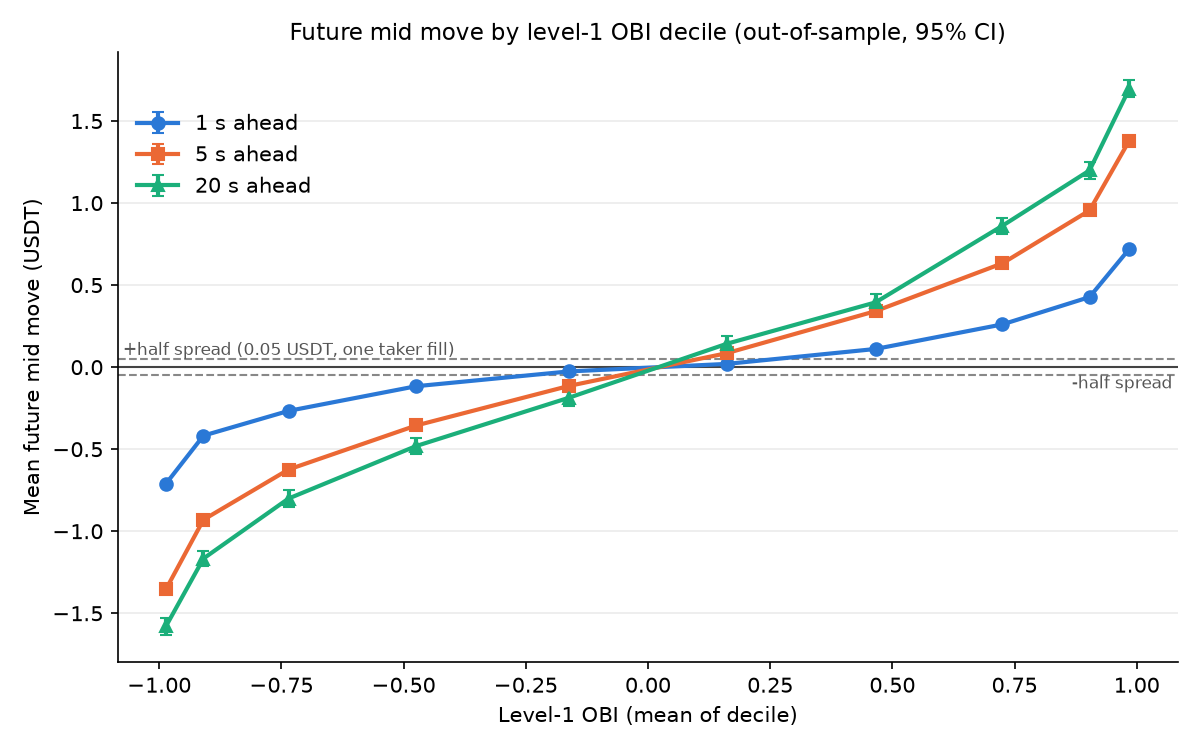
\includegraphics[width=0.8\textwidth]{obi_deciles.png}
\caption{Movimento medio del mid (USDT) nei secondi successivi, per decile di OBI di livello 1,
a 1, 5 e 20\,s, out-of-sample, con intervalli di confidenza al 95\%. Le linee tratteggiate
indicano $\pm s/2$, il costo di attraversare lo spread su un solo lato.}
\label{fig:obi-deciles}
\end{figure}

La Figura~\ref{fig:obi-deciles} guarda il fenomeno senza nessuna regola di trading, ed è il
grafico più convincente del progetto. Divido gli snapshot in dieci gruppi per valore dell'OBI e
misuro quanto si muove in media il mid dopo 1, 5 e 20\,s. La relazione è monotona: più il book
è sbilanciato verso il bid, più il prezzo sale, e viceversa. L'effetto si concentra nelle code:
nei decili estremi il mid si muove di circa 0.7\usdt{} a 1\,s e di oltre 1.5\usdt{} a 20\,s,
mentre a 1\,s i decili centrali restano quasi dentro la banda $\pm s/2$.

Il segnale quindi esiste. Lo spread non è l'ostacolo: nei decili estremi il movimento supera
nettamente uno spread intero (0.1\usdt{}). L'ostacolo sono le commissioni, che a 2\bp{} per
lato valgono circa 8\usdt{} per round trip.

\subsection{Ma non paga le commissioni}
\label{sec:ris-nonpaga}

\begin{table}[H]
\centering
\footnotesize
\caption{Strategia OBI, $\theta = 0.6$, out-of-sample. Win rate e t-stat a commissione nulla;
$f^*$ è la commissione di pareggio~\eqref{eq:breakeven}. Tutte le soglie e il confronto
in-sample sono nella Tabella~\ref{tab:obi-sweep} in appendice. Fonte: \code{obi\_sweep.csv}.}
\label{tab:obi-oos}
\begin{tabular}{@{}rrrrrrrrr@{}}
\toprule
Orizz. & Trade & Win rate & Mid move & EV lordo & t-stat & $f^*$ (bp) & EV netto 2\bp & EV netto 4\bp \\
\midrule
1\,s  & 163\,365 & 32.3\% & $+0.54$ & $+0.22$ & 45.0 & 0.05 & $-8.20$ & $-16.62$ \\
5\,s  & 46\,208  & 53.2\% & $+0.98$ & $+0.65$ & 32.6 & 0.15 & $-7.77$ & $-16.19$ \\
20\,s & 13\,134  & 56.0\% & $+1.21$ & $+0.90$ & 12.1 & 0.21 & $-7.51$ & $-15.93$ \\
60\,s & 4\,521   & 54.6\% & $+1.50$ & $+1.17$ & 5.3  & 0.28 & $-7.25$ & $-15.67$ \\
\bottomrule
\end{tabular}
\end{table}

La Tabella~\ref{tab:obi-oos} si legge da sinistra a destra.
\begin{itemize}[leftmargin=*]
  \item \textbf{Il segnale funziona}: l'EV lordo, che ha già pagato lo spread, è positivo a ogni
        orizzonte con t-stat tra 5 e 45. Lo stesso vale per tutte le soglie, in-sample e
        out-of-sample (t tra 3.6 e 57), e l'out-of-sample non è peggiore dell'in-sample.
  \item \textbf{Il win rate inganna}: a 1\,s è solo del 32\% eppure l'EV è positivo con
        $t = 45$. In un secondo il mid spesso non si muove, e chi è entrato all'ask ed esce al
        bid perde esattamente lo spread; quando invece il prezzo si muove, va più spesso nella
        direzione giusta.
  \item \textbf{Ma è piccolissimo}: $f^*$ va da 0.05 a 0.28\bp{}, contro 1.7--5\bp{} reali. A
        2\bp{} per lato si perdono circa 7--8\usdt{} per trade, a 4\bp{} circa 16.
\end{itemize}

\begin{figure}[H]
\centering
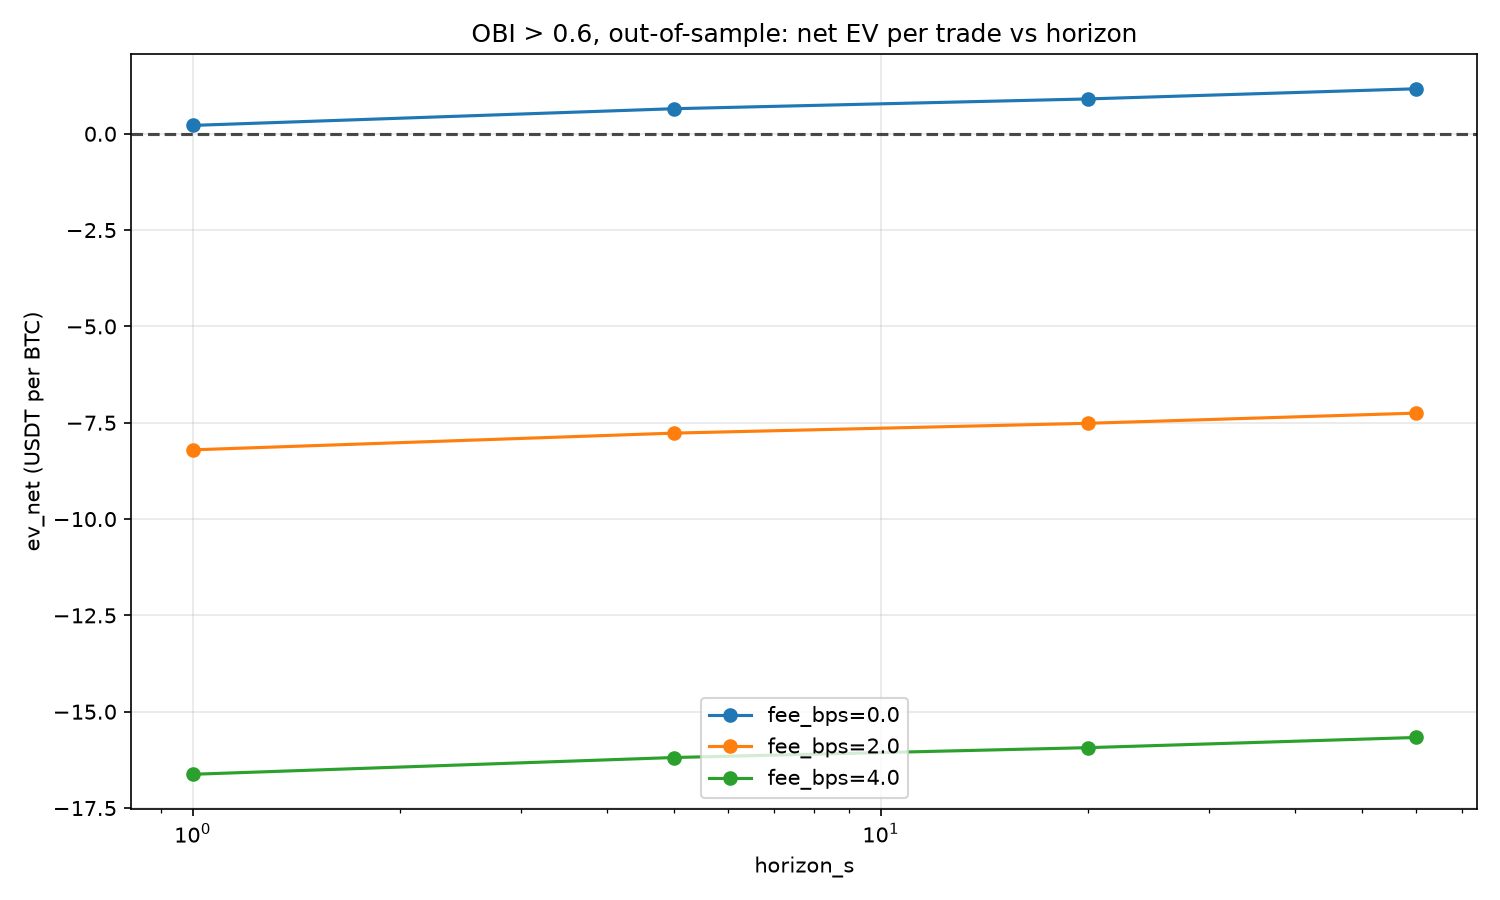
\includegraphics[width=0.75\textwidth]{obi_ev_decay.png}
\caption{OBI $>0.6$, out-of-sample: EV netto per trade in funzione dell'orizzonte (scala
logaritmica) per commissioni di 0, 2 e 4\bp{} per lato. La curva a 0\bp{} cresce con
l'orizzonte ma resta un ordine di grandezza sotto il costo delle commissioni.}
\label{fig:ev-decay}
\end{figure}

Un risultato mi ha sorpreso. Nella prima versione avevo parlato di ``alpha decay'': tenendo la
posizione più a lungo il vantaggio sembrava sparire. Con $\theta = 0.6$ l'EV lordo invece
\emph{cresce} con l'orizzonte, da 0.22\usdt{} a 1\,s a 1.17\usdt{} a 60\,s
(Figura~\ref{fig:ev-decay}). Su tutte le soglie, in-sample e out-of-sample, cresce fino a
20\,s; tra 20 e 60\,s continua a crescere in quattro casi su sei e cala leggermente negli altri
due (Tabella~\ref{tab:obi-sweep}).
Quello che peggiora allungando l'orizzonte è la significatività, perché ci sono meno trade e più
rumore. Il ``decadimento'' che vedevo era un effetto dei costi: con un costo fisso per trade gli
orizzonti brevi, dove il guadagno per trade è minimo, sono i più penalizzati.

\subsection{WOBI: stesso verdetto}
\label{sec:ris-wobi}

La strategia WOBI entra long se l'edge supera una soglia $\epsilon$ (in USDT) e
$\WOBI > 0.6$, short nel caso simmetrico. Esce con un bracket simmetrico: take-profit e
stop-loss alla stessa distanza dal fill (0.5, 1 o 2\usdt{}), con time-stop di 2.5\,s. Le
commissioni entrano nel PnL, non nel filtro di entrata.

\begin{table}[H]
\centering
\footnotesize
\caption{Strategia WOBI + micro-price con bracket TP/SL $=1$\usdt{}, out-of-sample. Win rate e
t-stat a commissione nulla; ``uscite'' è la quota di trade chiusi in take-profit / stop-loss /
time-stop. La griglia completa (TP/SL 0.5, 1, 2) è nella Tabella~\ref{tab:wobi-full} in
appendice. Fonte: \code{wobi\_sweep.csv}.}
\label{tab:wobi}
\begin{tabular}{@{}rrrrrrrr@{}}
\toprule
$\epsilon$ & Trade & Win rate & Mid move & EV lordo & t-stat & EV netto 4\bp & Uscite (\%) \\
\midrule
0.05 & 95\,998 & 52.7\% & 0.90 & 0.39 & 57.8 & $-16.46$ & 41/19/41 \\
0.10 & 46\,123 & 56.0\% & 1.14 & 0.36 & 30.9 & $-16.49$ & 46/24/30 \\
0.20 & 19\,796 & 55.5\% & 1.29 & 0.26 & 12.0 & $-16.59$ & 48/30/23 \\
\bottomrule
\end{tabular}
\end{table}

Il quadro è lo stesso dell'OBI (Tabella~\ref{tab:wobi}). Nella configurazione di riferimento ($\epsilon = 0.1$, TP/SL
$= 1$\usdt{}) ottengo 46\,123 trade, EV lordo $+0.36\usdt{}$ con $t \approx 31$ ed EV netto a
4\bp{} di $-16.5\usdt{}$. Su tutta la griglia la commissione di pareggio va da 0.05 a
0.11\bp{}, con valori in-sample e out-of-sample molto vicini.

Alzare $\epsilon$ aumenta il mid move ma non l'EV lordo. La mia interpretazione è che i segnali
più forti siano anche quelli che il mercato sconta più in fretta, per cui una parte del
movimento avviene durante i 250\,ms di latenza. Usare la profondità ha reso il segnale più
ordinato, ma non ne ha cambiato l'ordine di grandezza.

\subsection{Il costo della latenza}
\label{sec:ris-latenza}

Quest'ultima analisi non è una nuova strategia: riprendo l'OBI a orizzonte fisso e cambio solo
il ritardo del fill. Uso l'orizzonte fisso e non il bracket perché, cambiando la latenza,
cambierebbero anche le uscite in take-profit e stop-loss, e non potrei isolare l'effetto del
ritardo.

\begin{table}[H]
\centering
\small
\caption{EV lordo in funzione della latenza; OBI $\theta=0.6$, out-of-sample; tra parentesi la
variazione rispetto a latenza nulla. Grafico in Figura~\ref{fig:latency-decay} in appendice.
Fonte: \code{latency\_sweep.csv}.}
\label{tab:latenza}
\begin{tabular}{@{}rcc@{}}
\toprule
Latenza & EV lordo a 1\,s & EV lordo a 5\,s \\
\midrule
0\,ms (irrealistico) & 0.37 & 0.84 \\
250\,ms  & 0.22 ($-41\%$) & 0.65 ($-23\%$) \\
500\,ms  & 0.15 ($-60\%$) & 0.55 ($-35\%$) \\
1000\,ms & 0.10 ($-73\%$) & 0.42 ($-50\%$) \\
\bottomrule
\end{tabular}
\end{table}

A 1\,s, passare da 0 a 250\,ms costa il 41\% dell'EV lordo, e a 1000\,ms ne resta poco più di
un quarto. A 5\,s la perdita è più lenta, perché una parte maggiore del movimento avviene dopo
il primo secondo. Buona parte dell'informazione entra nel prezzo subito dopo il segnale: chi
arriva tardi paga lo spread per un movimento già avvenuto. Questo spiega anche perché il backtest
a latenza zero della prima versione era così ottimista.

% ---------------------------------------------------------------------------
\section{Cosa avevo sbagliato nella prima versione}
\label{sec:v1}

I risultati precedenti vengono da una seconda versione del progetto. La prima (ancora nel
repository, in \code{legacy/}) seguiva le stesse due idee, OBI e poi WOBI, ma con un
backtest molto diverso e un risultato molto più bello.

\subsection{Il miraggio del 90\%}

Il primo backtest dell'OBI girava sulle prime 100\,000 righe (circa 7 ore, tutte in-sample),
eseguiva ai prezzi dello stesso snapshot che generava il segnale, contava gli orizzonti in
snapshot (4, 20 e 80, che interpretavo come 1, 5 e 20\,s), non aveva commissioni e sottraeva
solo uno ``slippage'' fisso. Ne usciva un win rate sopra il 90\%.

Non ci ho creduto, e il motivo è più da giocatore di poker che da ingegnere. Al tavolo non
basta vincere spesso: una mano va giocata se il piatto paga abbastanza rispetto a quanto costa
restare dentro, cioè se le \emph{pot odds} sono favorevoli. Un win rate del 90\% su movimenti
di un tick, con uno spread di un tick da pagare, non aveva senso. Ho smesso di guardare il win
rate e ho iniziato a ragionare in termini di valore atteso al netto dei costi.

Quel 90\% non sono più riuscito a riprodurlo: non ho più il codice né la configurazione che
l'avevano prodotto. Rieseguendo il metodo originale ancora presente nel repository (prime
100\,000 righe, latenza zero, nessuna commissione) ottengo un win rate tra il 15\% e il 55\%
(Tabella~\ref{tab:legacy}), e già 0.5\usdt{} di slippage per round trip rendono negativo l'EV a
1 e 5\,s. Lo considero un dato inaffidabile e non ci costruisco sopra nessuna conclusione.

\begin{table}[H]
\centering
\footnotesize
\caption{Metodo originale rieseguito (prime 100k righe, $\theta=0.6$, latenza 0, nessuna
commissione, volumi corretti). ``Slip.'' è l'EV per uno slippage di round trip di 0.5, 1 e
2\usdt{}. Con i volumi troncati a intero i numeri sono quasi identici
(Tabella~\ref{tab:legacy-full}). Fonte: \code{obi\_legacy\_method.csv}.}
\label{tab:legacy}
\begin{tabular}{@{}lrrrrrrr@{}}
\toprule
Orizz. & Trade & Win rate & Mid move & EV lordo & slip.\ 0.5 & slip.\ 1 & slip.\ 2 \\
\midrule
1\,s  & 15\,018 & 15.0\% & 0.13 & 0.034 & $-0.466$ & $-0.966$ & $-1.966$ \\
5\,s  & 3\,582  & 38.4\% & 0.45 & 0.348 & $-0.152$ & $-0.652$ & $-1.652$ \\
20\,s & 1\,065  & 54.8\% & 0.84 & 0.740 & $0.240$  & $-0.260$ & $-1.260$ \\
\bottomrule
\end{tabular}
\end{table}

\subsection{Gli errori}

Rileggendo tutto il codice per capire perché certi numeri non tornavano ho trovato più errori
di quanti mi aspettassi.

\paragraph{Volumi troncati a intero.} Il motore C memorizzava i volumi come interi. Il volume
al touch è sotto 1\,BTC in circa il 14\% degli snapshot per lato, e lì il troncamento lo
azzerava: 0.3 contro 0.7\,BTC diventava 0 contro 0 (OBI $=0$ invece di $-0.4$), 1.2 contro 0.7
diventava 1 contro 0 (OBI $=+1$). Così il 26.5\% degli snapshot aveva OBI esattamente $\pm1$,
contro lo 0\% con i volumi corretti (Tabella~\ref{tab:obi-dist}). Nel grafico che avevo fatto
allora (Figura~\ref{fig:price-obi}, qui ricalcolata con i volumi corretti) l'OBI sembrava
``saturare'' di continuo mentre il prezzo restava fermo, e io l'avevo letto come una proprietà
del mercato: era in buona parte un mio bug. Sulla
soglia 0.6 il backtest cambia poco, perché la quota di snapshot con $|\OBI| > 0.6$ è quasi la
stessa, ma l'informazione graduale del segnale va persa.

\begin{table}[H]
\centering
\small
\caption{Distribuzione dell'OBI di livello 1 sull'intero dataset con volumi corretti e troncati
a intero (istogramma in Figura~\ref{fig:obi-dist} in appendice). Fonte:
\code{obi\_signal\_distribution.csv}.}
\label{tab:obi-dist}
\begin{tabular}{@{}lrr@{}}
\toprule
Metrica & Corretto (float) & Prima versione (int) \\
\midrule
Quota con $|\OBI| = 1$     & 0.00\%  & 26.50\% \\
Quota con $|\OBI| > 0.6$   & 61.12\% & 62.33\% \\
Quota con $\OBI = 0$       & 0.005\% & 2.19\%  \\
Media di $|\OBI|$          & 0.652   & 0.674   \\
\bottomrule
\end{tabular}
\end{table}

\begin{figure}[H]
\centering
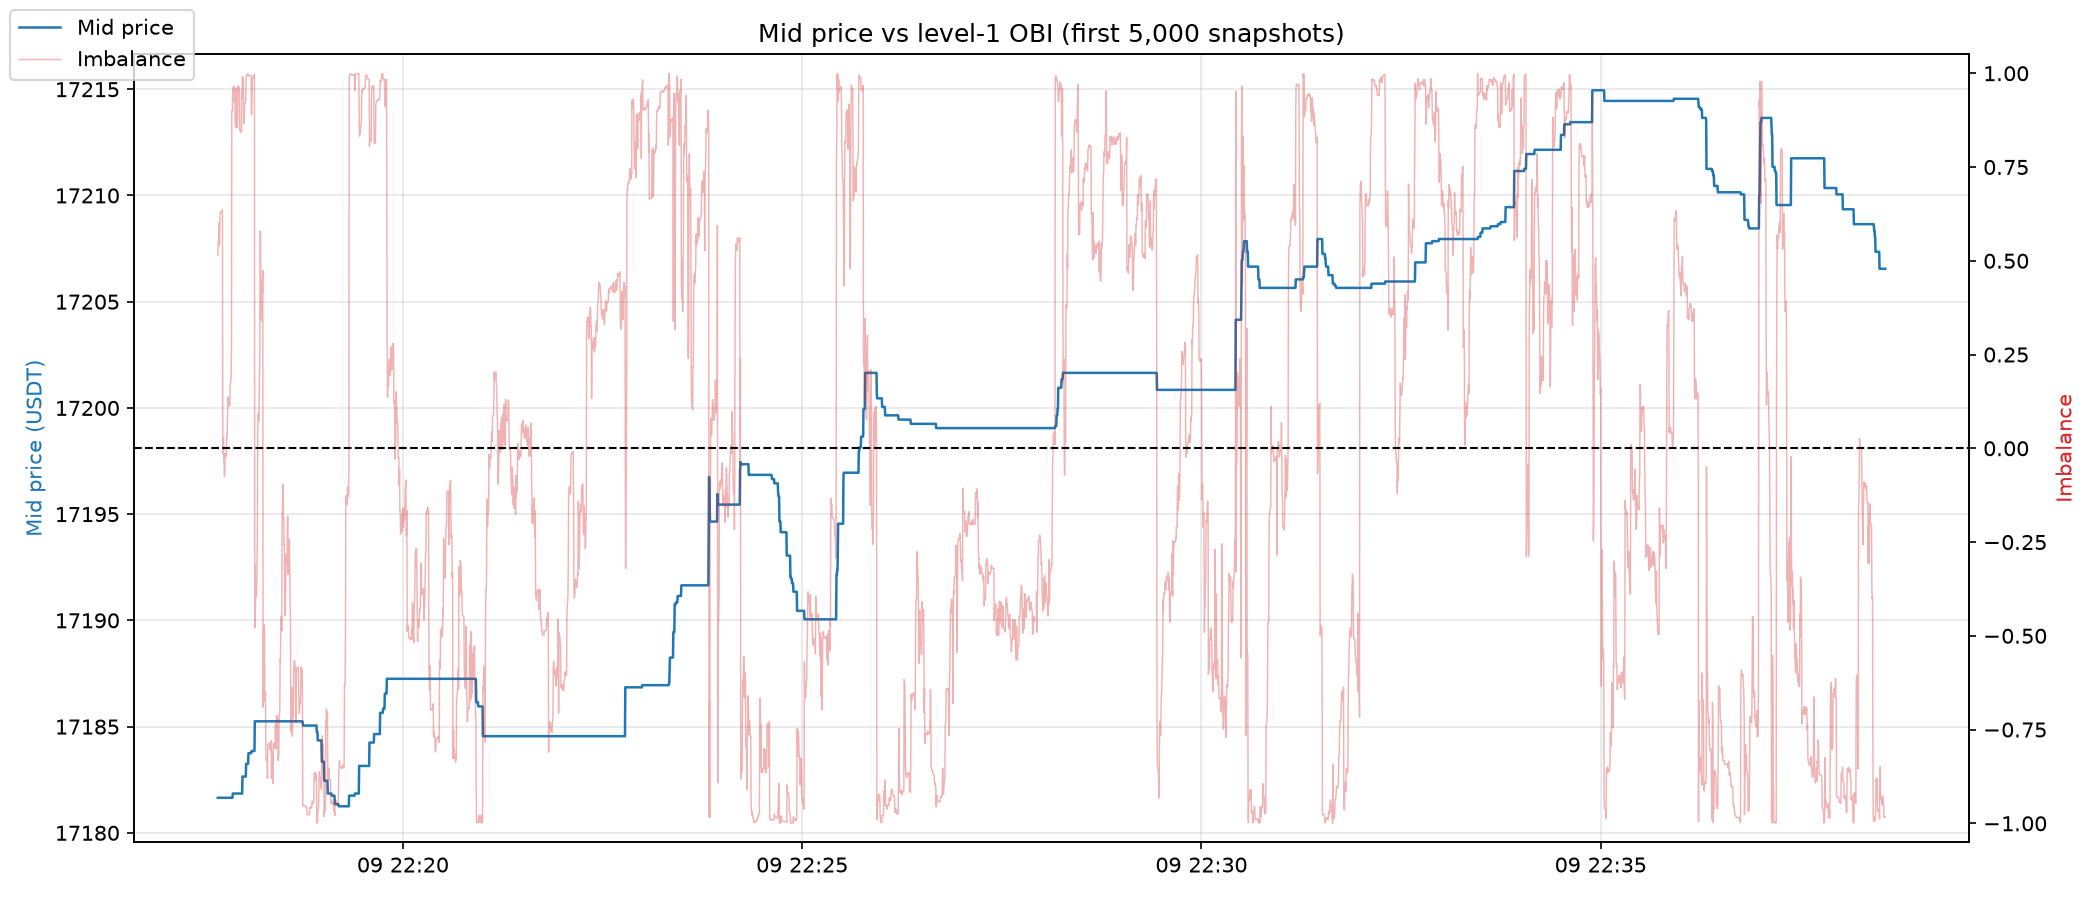
\includegraphics[width=\textwidth]{price_vs_obi.png}
\caption{Mid-price (blu, asse sinistro) e OBI di livello 1 (rosso, asse destro) sui primi
5\,000 snapshot, ricalcolato con i volumi corretti. Anche così l'OBI oscilla spesso tra valori
estremi mentre il mid resta fermo per decine di secondi.}
\label{fig:price-obi}
\end{figure}

\paragraph{Un filtro WOBI con unità miste.} La prima strategia WOBI entrava long se
$e > 0.2 + s + m\cdot 0.0004$: sommava a soglia e spread la commissione di un lato,
$m \cdot 0.0004 \approx 8\usdt{}$, e confrontava il tutto con un edge che non supera quasi mai
1\usdt{}. La condizione era vera su 5 snapshot su 3.73 milioni: la strategia di fatto non
faceva trade, e io non me ne ero accorto perché guardavo statistiche aggregate e non il numero
di operazioni.

\paragraph{Take-profit sotto il pareggio.} Il take-profit era fissato al micro-price calcolato
all'ingresso, che copriva al più la commissione di entrata; in uscita ne pagavo una seconda,
quindi anche i trade chiusi in take-profit erano in perdita. Ora take-profit e stop-loss sono
distanze in USDT dal prezzo di fill.

\paragraph{Un finto modello di EV.} Lo script di ingestione stimava un ``valore atteso'' con
una probabilità di successo inventata, $p = 0.5 + 0.2\,|\OBI|$, guadagno fisso 2\usdt{},
perdita fissa 1\usdt{} e slippage 0.5\usdt{}. Il conto dà $\EV = 0.6\,|\OBI|$, quindi la
condizione ``segnale profittevole'' $\EV > 0.1$ equivaleva a $|\OBI| > 1/6$: stavo solo contando
gli snapshot sopra una soglia implicita, senza nessun parametro stimato dai dati.

\paragraph{Metodologia.} Il resto erano scelte ingenue più che bug: latenza zero, nessuna
commissione nel backtest OBI, solo dati in-sample, e orizzonti contati in snapshot. Sulle prime
100\,000 righe i buchi nei dati sono brevi, ma sul dataset completo, con buchi fino a 93\,s, un
trade ``da 1\,s'' contato in snapshot poteva durare più di un minuto. Nel README di allora
avevo anche scritto di sfruttare il multithreading, ma il codice non lo faceva.

Invece di correggere gli script uno per uno ho riscritto la pipeline attorno a un unico motore
di backtest con le regole esplicite della Sezione~\ref{sec:esecuzione}, e con un test di
regressione per ciascuno di questi errori.

% ---------------------------------------------------------------------------
\section{Limiti e prossimi passi}
\label{sec:limiti}

Il limite principale non è nel codice: un edge di frazioni di punto base contro commissioni
taker di 1.7--5\bp{} è un divario che va da circa 5 volte, nel caso più favorevole, a circa
130 volte per un conto standard, e nessuna scelta di soglia, orizzonte o bracket lo colma. È la
conclusione che considero più solida.

Il secondo limite sono i dati. Snapshot ogni 250\,ms senza il flusso dei trade non dicono cosa
succede tra uno snapshot e l'altro, né quale sarebbe la mia posizione in coda con un ordine
limite. Per questo il market making, l'uso che mi sembra più promettente per questo segnale,
con questi dati non è testabile in modo credibile: il risultato dipenderebbe quasi solo dalle
ipotesi sul fill. Lavoro poi su un solo strumento, 11 giorni e circa 3 giorni di
out-of-sample, con un solo split. La statistica è ingenua: trade consecutivi sono
autocorrelati e ho guardato 21 configurazioni senza correzione per test multipli. Con t-stat
fino a 50--60 sugli orizzonti brevi non credo che ``il segnale esiste'' cambierebbe, ma la
significatività è sovrastimata.

I passi successivi, in ordine di priorità:
\begin{enumerate}[leftmargin=*]
  \item Dati L2 incrementali (le singole modifiche del book) insieme ai trade, con timestamp
        dell'exchange, su più mesi e più strumenti.
  \item Un simulatore a eventi con coda FIFO per livello e fill sui trade reali: l'unico modo
        per testare seriamente l'esecuzione passiva.
  \item Usare il segnale per il pricing e non per la direzione, per esempio quote asimmetriche
        o gestione dell'inventario alla Avellaneda--Stoikov con un drift stimato
        dall'imbalance. Con commissioni maker nulle o negative, un edge di
        qualche decimo di punto base diventa rilevante.
  \item Feature migliori (Order Flow Imbalance, micro-price di Stoikov) valutate con $R^2$
        out-of-sample invece di soglie fisse.
  \item Validazione walk-forward, errori standard robusti all'autocorrelazione (Newey--West o
        bootstrap a blocchi) e una correzione per test multipli come il deflated Sharpe
        ratio.
\end{enumerate}

\subsection{Letture da cui ripartirei}
\label{sec:letture}

Questi sono i lavori di riferimento sui temi toccati dal report. Non li ho ancora studiati: li
elenco come punto di partenza per i prossimi passi, non come fonti delle affermazioni fatte qui.
\begin{itemize}[leftmargin=*]
  \item R.~Cont, A.~Kukanov e S.~Stoikov, \emph{The price impact of order book events},
        Journal of Financial Econometrics, 2014. Come gli eventi al touch del book muovono il
        prezzo; introduce l'Order Flow Imbalance.
  \item S.~Stoikov, \emph{The micro-price: a high-frequency estimator of future prices},
        Quantitative Finance, 2018. La definizione di micro-price stimata dai dati.
  \item M.~Avellaneda e S.~Stoikov, \emph{High-frequency trading in a limit order book},
        Quantitative Finance, 2008. Il modello classico di market making con gestione
        dell'inventario.
  \item Á.~Cartea, S.~Jaimungal e J.~Penalva, \emph{Algorithmic and High-Frequency Trading},
        Cambridge University Press, 2015. Manuale su microstruttura, esecuzione e market
        making.
  \item D.~H.~Bailey e M.~López de Prado, \emph{The deflated Sharpe ratio: correcting for
        selection bias, backtest overfitting, and non-normality}, Journal of Portfolio
        Management, 2014. Una correzione per test multipli nei backtest.
\end{itemize}

% ---------------------------------------------------------------------------
\section{Conclusioni}
\label{sec:conclusioni}

Sono partito da un'idea semplice e da un numero troppo bello, che non sono più riuscito a
riprodurre, e il lavoro più utile è stato non fidarmi di quel numero e rifare l'analisi da capo.
Corretti gli errori, il quadro è chiaro: l'imbalance del book, al livello 1 come su dieci
livelli, predice il movimento del mid tra 1 e 60 secondi, anche out-of-sample; ma l'edge vale
0.04--0.3\bp{} per lato, uno o due ordini di grandezza sotto le commissioni taker, ed è eroso
rapidamente dalla latenza.

La lezione che mi porto dietro è quella che avevo intuito pensando alle pot odds: la probabilità
di avere ragione conta solo insieme al prezzo che si paga per giocare. L'imbalance mi sembra
un'informazione utile per decidere \emph{come} quotare più che \emph{se} attraversare lo spread,
ma verificarlo richiede dati a livello di evento e un simulatore di esecuzione passiva, ed è da
lì che vorrei ripartire.

\paragraph{Nota sugli strumenti.} Ho usato assistenti AI per parte del refactoring del codice,
per scrivere alcuni test e nella stesura di questo testo; la domanda di ricerca, le scelte di
analisi e le conclusioni sono mie.

% ---------------------------------------------------------------------------
\appendix

\section{Motore di calcolo e benchmark}
\label{app:calcolo}

Iterare 3.7 milioni di righe in Python rendeva ogni prova lentissima, quindi ho separato il
calcolo dei segnali, in C, dall'analisi, in Python. Il motore (\code{engine/include/lob\_engine.h})
elabora $n$ snapshot per chiamata e parallelizza sulle righe con OpenMP; ogni riga è calcolata
da un solo thread, quindi il risultato non dipende dal numero di thread. Gli snapshot sono righe
di 40 double nello stesso ordine del CSV, così l'array NumPy passa al C senza copie via
\code{ctypes}, con una chiamata per dataset invece che una per tick come nel codice originale.
Il CSV è letto una volta e salvato in una cache \code{.npy} aperta in memory-map. Per fidarmi
del C l'ho confrontato con un'implementazione indipendente in NumPy con tolleranza $10^{-12}$.

% Generated by scripts/benchmarks_to_latex.py from results/benchmarks.json.
% Generated by scripts/benchmarks_to_latex.py from results/benchmarks.json.
% Do not edit by hand: re-run the script after scripts/run_benchmarks.py.

Ho misurato le prestazioni con \texttt{scripts/run\_benchmarks.py} e ho fissato delle soglie
di regressione in \texttt{pytest -m bench}, così se una modifica peggiora i tempi me ne accorgo.
Salvo dove indicato, ho usato l'intero dataset (3\,730\,870 snapshot,
1{,}19\,GB in \texttt{float64}) già caricato in RAM.

\paragraph{Ambiente di misura.} Il mio portatile: CPU Intel Core Ultra 7 155H
(22 thread OpenMP), Windows 11,
compilatore gcc (MinGW-w64) con \texttt{-O3 -march=native -fopenmp},
Python 3.13.9, NumPy 2.5.3, motore v1.0.0.
Per i tempi riporto il migliore su più ripetizioni; per le latenze delle singole chiamate
riporto i percentili su centinaia di migliaia di chiamate.

\subsection{Calcolo dei segnali sull'intero dataset}

Nella Tabella~\ref{tab:bench-headline} confronto il mio codice originale, che attraversava il
confine Python/C una o due volte per ogni snapshot, con l'API batch, che passa l'intero
array al motore C in una sola chiamata.

\begin{table}[H]
\centering
\caption{Tempo per calcolare i segnali su tutti gli snapshot.}
\label{tab:bench-headline}
\begin{tabular}{p{7.2cm}rrr}
\toprule
Percorso & Tempo totale (s) & ns/snapshot & vs originale \\
\midrule
Script OBI originale (\texttt{csv.reader} + 2 chiamate ctypes per tick) & 24{,}6 & 6\,582 & 1{,}0$\times$ \\
Loop WOBI originale (40 scritture ctypes + 1 chiamata per tick) & 34{,}1 & 9\,132 & 0{,}7$\times$ \\
WOBI vettoriale NumPy (1 thread) & 0{,}972 & 261 & 25$\times$ \\
WOBI batch in C, 1 thread & 0{,}087 & 23{,}4 & 282$\times$ \\
\textbf{WOBI batch in C, 22 thread} & 0{,}028 & 7{,}6 & 872$\times$ \\
\bottomrule
\end{tabular}
\end{table}

Il mio script originale impiega 24{,}6\,s sul CSV completo (nel primo
README avevo scritto circa 22\,s). Profilandolo ho capito che quasi tutto quel tempo era
interprete Python e marshalling ctypes, non calcolo: il C che avevo scritto pesava pochissimo.
Con il batch lo stesso lavoro scende a
28\,ms, un fattore
872.

\subsection{Scalabilità OpenMP}

\begin{table}[H]
\centering
\caption{Kernel batch in C al variare del numero di thread (dati già in RAM).}
\label{tab:bench-scaling}
\small\setlength{\tabcolsep}{4pt}
\begin{tabular}{rrrrrrr}
\toprule
Thread & OBI ns/riga & Speedup & WOBI ns/riga & Mrighe/s & Speedup & Efficienza \\
 & & OBI & & WOBI & WOBI & WOBI \\
\midrule
1 & 23{,}14 & 1{,}0$\times$ & 23{,}35 & 43 & 1{,}0$\times$ & 100\,\% \\
2 & 11{,}13 & 2{,}1$\times$ & 14{,}24 & 70 & 1{,}6$\times$ & 82\,\% \\
4 & 6{,}01 & 3{,}8$\times$ & 9{,}96 & 100 & 2{,}3$\times$ & 59\,\% \\
8 & 4{,}00 & 5{,}8$\times$ & 8{,}89 & 112 & 2{,}6$\times$ & 33\,\% \\
12 & 3{,}73 & 6{,}2$\times$ & 7{,}79 & 128 & 3{,}0$\times$ & 25\,\% \\
16 & 3{,}84 & 6{,}0$\times$ & 7{,}69 & 130 & 3{,}0$\times$ & 19\,\% \\
22 & 3{,}85 & 6{,}0$\times$ & 7{,}55 & 132 & 3{,}1$\times$ & 14\,\% \\
\bottomrule
\end{tabular}
\end{table}

\begin{figure}[H]
\centering
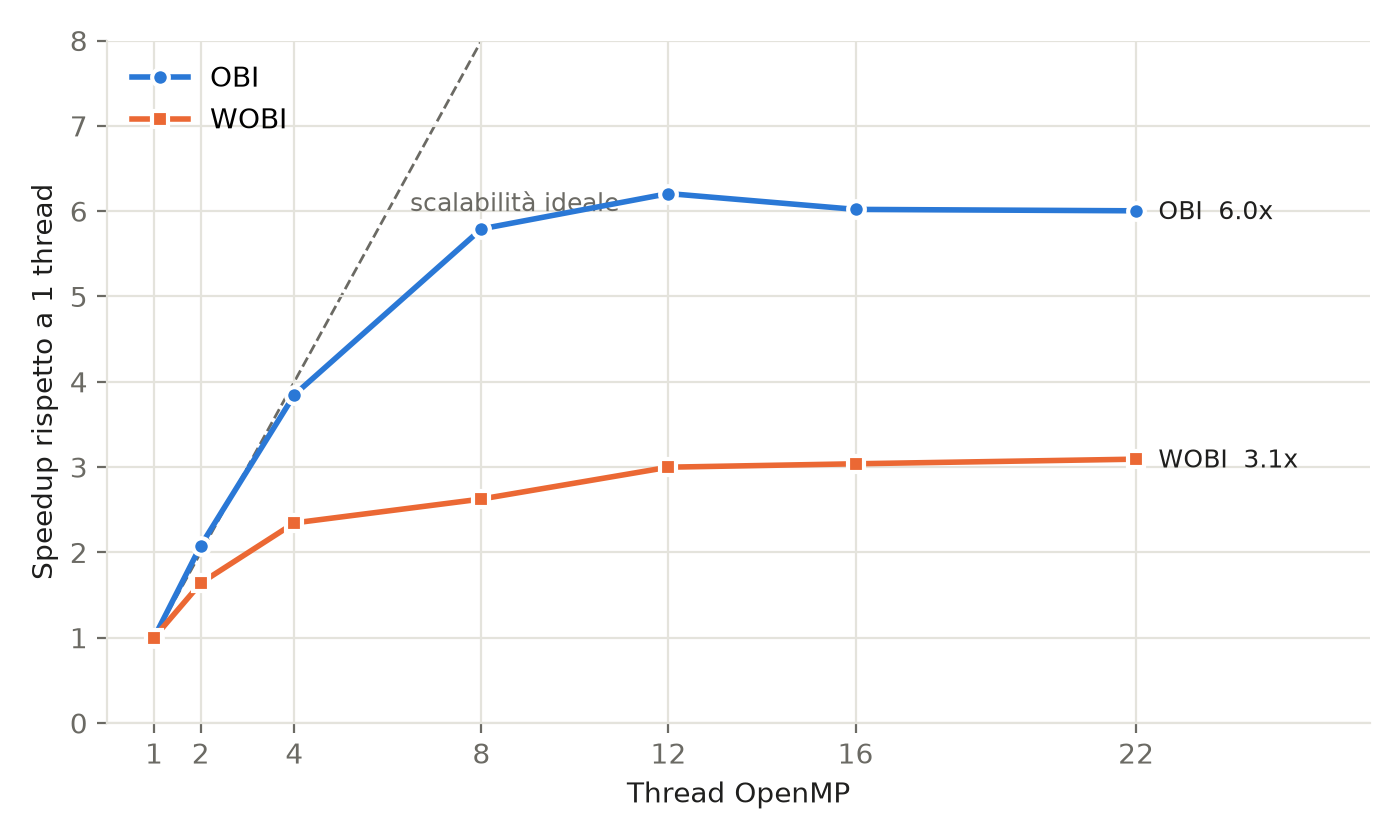
\includegraphics[width=0.8\textwidth]{openmp_scaling.png}
\caption{Speedup dei kernel batch rispetto a un thread. La linea tratteggiata è la
scalabilità lineare ideale.}
\label{fig:bench-scaling}
\end{figure}

La scalabilità si appiattisce presto (Figura~\ref{fig:bench-scaling}): con
22 thread lo speedup è 6{,}0$\times$ per OBI e
3{,}1$\times$ per WOBI. Ogni snapshot occupa 320 byte ma i kernel
eseguono poche operazioni per byte letto (OBI usa 16 byte su 320), quindi il limite è la
banda di memoria e non il numero di core. Il margine residuo sta nel layout dei dati
(colonne separate, precisione ridotta), non in più thread.

\subsection{Latenza per snapshot (tick-to-signal)}

Un sistema live riceve uno snapshot alla volta e deve produrre il segnale subito, quindi ho
misurato anche il costo di una singola chiamata (Tabella~\ref{tab:bench-latency}).

\begin{table}[H]
\centering
\caption{Latenza per singolo snapshot, in nanosecondi (massimo in microsecondi).}
\label{tab:bench-latency}
\begin{tabular}{p{6.2cm}rrrr}
\toprule
Percorso & p50 & p99 & p99{,}9 & max ($\mu$s) \\
\midrule
Solo C, \texttt{lob\_obi\_one} & 16 & 317 & 547 & 1\,699 \\
Solo C, \texttt{lob\_wobi\_one} & 21 & 62 & 81 & 1\,854 \\
Python $\to$ ctypes $\to$ \texttt{lob\_obi\_one} & 300 & 800 & 1\,200 & 1\,853 \\
Python $\to$ ctypes $\to$ \texttt{lob\_wobi\_one} & 1\,000 & 2\,700 & 11\,000 & 2\,931 \\
WOBI originale per tick & 7\,200 & 19\,100 & 94\,802 & 7\,287 \\
\bottomrule
\end{tabular}
\end{table}

Il kernel WOBI in C costa circa 21\,ns (misurati con il
contatore TSC del processore, overhead del timer 17\,ns
incluso). Chiamato da Python la mediana sale a 1\,000\,ns, circa
48 volte di più: il costo è il confine Python/ctypes, non il calcolo.
Per le misure lato Python ho dovuto usare \texttt{perf\_counter\_ns}, che su Windows ha
risoluzione di 100\,ns, quindi quei valori sono quantizzati a quel passo. I massimi, nell'ordine dei millisecondi, sono dovuti
a preemption del sistema operativo e interrupt, non al codice.

\subsection{Caricamento dei dati e pipeline completa}

\begin{table}[H]
\centering
\caption{Caricamento dei dati e pipeline di ricerca end-to-end sull'intero dataset.}
\label{tab:bench-e2e}
\begin{tabular}{lr}
\toprule
Passo & Tempo \\
\midrule
Parsing del CSV grezzo (una tantum, \texttt{prepare\_data.py}) & circa 13\,s \\
Apertura della cache \texttt{.npy} memory-mapped & 1{,}2\,ms \\
Caricamento completo della cache in RAM & 0{,}56\,s \\
\midrule
Segnale OBI (batch C, da memory-map) & 164\,ms \\
WOBI e micro-price (batch C) & 133\,ms \\
Backtest OBI a orizzonte fisso (541\,959 trade) & 0{,}84\,s \\
Backtest WOBI con bracket (62\,921 trade) & 0{,}63\,s \\
\midrule
\textbf{Totale pipeline} & \textbf{1{,}77\,s} \\
\bottomrule
\end{tabular}
\end{table}

Una volta ridotti i segnali a decine di millisecondi, il collo di bottiglia è diventato il
backtest, che itera in Python una volta per trade. Rendendo vettoriale il calcolo di ingressi,
uscite e PnL ho portato il backtest OBI da 5{,}2\,s a meno di 1\,s, con gli stessi trade
selezionati.

\subsection{Sintesi}

\begin{itemize}[leftmargin=*]
\item Il calcolo dei segnali non è più un collo di bottiglia: 872 volte
più veloce del codice originale sull'intero dataset.
\item I kernel batch sono limitati dalla banda di memoria; il prossimo guadagno viene dal
layout dei dati, non da più thread.
\item Nel percorso per singolo tick oltre il 95\,\% del tempo è overhead Python/ctypes;
un sistema live dovrebbe tenere l'intero percorso critico in C/C++.
\end{itemize}


\section{Tabelle e figure complete}
\label{app:tabelle}

\IfFileExists{data_summary.tex}{% Generated by scripts/describe_data.py from results/data_summary.json.
% Do not edit by hand: re-run the script after changing the dataset.
\begin{table}[H]
\centering
\caption{Statistiche descrittive del dataset BTC/USDT (\texttt{1-09-1-20.csv}): snapshot
del book a 10 livelli, campionati ogni 250 ms nominali.}
\label{tab:data-summary}
\small
\begin{tabular}{p{0.43\linewidth}p{0.47\linewidth}}
\toprule
Grandezza & Valore \\
\midrule
Periodo (UTC) & 09/01/2023 22:17:40 -- 20/01/2023 18:10:48 \\
Durata & 259{,}9 ore (10{,}8 giorni) \\
Snapshot & 3\,730\,870 \\
\midrule
Intervallo tra snapshot: mediana / p99 & 250 / 254 ms \\
Interruzioni (gap) $>$ 500 ms / $>$ 2 s & 296 / 136 \\
Gap massimo & 93{,}5 s \\
\midrule
Prezzo medio (mid): min / max & 17\,118{,}35 / 21\,659{,}85 USDT \\
Spread: mediana / media & 0{,}10 / 0{,}108 USDT \\
Spread: p99 / p99,9 / max & 0{,}10 / 1{,}80 / 161{,}0 USDT \\
Quota di spread pari a 1 tick (0,1 USDT) & 99{,}2\% \\
\midrule
Volume al best bid: mediana / media & 11{,}08 / 17{,}67 BTC \\
Volume al best ask: mediana / media & 10{,}78 / 17{,}32 BTC \\
Volume al best level $<$ 0,01 BTC (bid / ask) & 0{,}70\% / 0{,}67\% \\
Volume al best level $<$ 1 BTC (bid / ask) & 14{,}0\% / 13{,}9\% \\
Volume totale 10 livelli, bid: mediana / media & 19{,}9 / 29{,}7 BTC \\
Volume totale 10 livelli, ask: mediana / media & 19{,}5 / 29{,}2 BTC \\
\midrule
OBI livello 1: media di $|\mathrm{OBI}|$ & 0{,}652 \\
Quota con $|\mathrm{OBI}| > 0{,}6$ / $|\mathrm{OBI}| = 1$ & 61{,}1\% / 0{,}0\% \\
\midrule
In-sample (70\%) & 2\,611\,609 snapshot, fino al 17/01/2023 12:11:56 \\
Out-of-sample (30\%) & 1\,119\,261 snapshot, dal 17/01/2023 12:11:56 \\
Controlli di coerenza & nessun problema (book incrociati: 0, NaN: 0, timestamp non crescenti: 0) \\
\bottomrule
\end{tabular}
\end{table}
}{}

\begin{table}[H]
\centering
\small
\caption{Strategia OBI: EV lordo in USDT per trade (t-stat tra parentesi) per soglia e
orizzonte, in-sample (IS) e out-of-sample (OOS). Fonte: \code{obi\_sweep.csv}.}
\label{tab:obi-sweep}
\begin{tabular}{@{}llccc@{}}
\toprule
Campione & Orizz. & $\theta=0.4$ & $\theta=0.6$ & $\theta=0.8$ \\
\midrule
IS  & 1\,s  & 0.15 (47.2) & 0.18 (51.0) & 0.24 (57.2) \\
IS  & 5\,s  & 0.46 (32.9) & 0.53 (35.1) & 0.65 (38.2) \\
IS  & 20\,s & 0.55 (10.2) & 0.76 (13.6) & 0.77 (13.4) \\
IS  & 60\,s & 0.59 (3.7)  & 0.72 (4.3)  & 1.10 (6.6)  \\
\midrule
OOS & 1\,s  & 0.17 (39.4) & 0.22 (45.0) & 0.27 (48.4) \\
OOS & 5\,s  & 0.58 (30.8) & 0.65 (32.6) & 0.73 (33.3) \\
OOS & 20\,s & 0.82 (11.2) & 0.90 (12.1) & 1.02 (13.4) \\
OOS & 60\,s & 0.78 (3.6)  & 1.17 (5.3)  & 1.30 (5.9)  \\
\bottomrule
\end{tabular}
\end{table}

\begin{table}[H]
\centering
\footnotesize
\caption{Strategia WOBI + micro-price ($D=10$, $\alpha=0.5$, $\WOBI > 0.6$, time-stop 2.5\,s),
griglia completa, out-of-sample. $\epsilon$: soglia sull'edge (USDT); TP/SL: bracket simmetrico
(USDT); win rate e t-stat a commissione nulla; uscite: quota tp/sl/time in \%; hold: durata
media (s); ultima colonna: EV lordo in-sample. Fonte: \code{wobi\_sweep.csv}.}
\label{tab:wobi-full}
\setlength{\tabcolsep}{4pt}
\begin{tabular}{@{}rrrrrrrrcrr@{}}
\toprule
$\epsilon$ & TP/SL & Trade & Win & Mid & EV & t-stat & EV netto & Uscite & Hold & EV lordo \\
 & & & rate & move & lordo & & 4\bp & tp/sl/time & (s) & IS \\
\midrule
0.05 & 0.5 & 107\,100 & 54.1\% & 0.87 & 0.34 & 58.9 & $-16.51$ & 49/20/32 & 1.39 & 0.32 \\
0.05 & 1.0 & 95\,998  & 52.7\% & 0.90 & 0.39 & 57.8 & $-16.46$ & 41/19/41 & 1.58 & 0.36 \\
0.05 & 2.0 & 82\,697  & 51.1\% & 0.95 & 0.45 & 54.0 & $-16.39$ & 26/15/59 & 1.92 & 0.40 \\
0.10 & 0.5 & 49\,411  & 57.1\% & 1.09 & 0.31 & 29.7 & $-16.55$ & 53/25/22 & 1.15 & 0.30 \\
0.10 & 1.0 & 46\,123  & 56.0\% & 1.14 & 0.36 & 30.9 & $-16.49$ & 46/24/30 & 1.35 & 0.35 \\
0.10 & 2.0 & 41\,308  & 54.6\% & 1.20 & 0.43 & 30.0 & $-16.42$ & 33/21/47 & 1.70 & 0.40 \\
0.20 & 0.5 & 20\,430  & 56.0\% & 1.23 & 0.19 & 9.9  & $-16.65$ & 53/31/16 & 0.98 & 0.21 \\
0.20 & 1.0 & 19\,796  & 55.5\% & 1.29 & 0.26 & 12.0 & $-16.59$ & 48/30/23 & 1.15 & 0.26 \\
0.20 & 2.0 & 18\,651  & 54.5\% & 1.38 & 0.34 & 13.4 & $-16.51$ & 37/27/36 & 1.48 & 0.31 \\
\bottomrule
\end{tabular}
\end{table}

\begin{table}[H]
\centering
\footnotesize
\caption{Metodo originale rieseguito con volumi corretti (float) e troncati a intero come nella
prima versione (int). Stesse condizioni della Tabella~\ref{tab:legacy}. Fonte:
\code{obi\_legacy\_method.csv}.}
\label{tab:legacy-full}
\begin{tabular}{@{}llrrrrrrr@{}}
\toprule
Volumi & Orizz. & Trade & Win rate & Mid move & EV lordo & slip.\ 0.5 & slip.\ 1 & slip.\ 2 \\
\midrule
float & 1\,s  & 15\,018 & 15.0\% & 0.13 & 0.034 & $-0.466$ & $-0.966$ & $-1.966$ \\
float & 5\,s  & 3\,582  & 38.4\% & 0.45 & 0.348 & $-0.152$ & $-0.652$ & $-1.652$ \\
float & 20\,s & 1\,065  & 54.8\% & 0.84 & 0.740 & $0.240$  & $-0.260$ & $-1.260$ \\
\midrule
int   & 1\,s  & 15\,200 & 14.9\% & 0.13 & 0.032 & $-0.468$ & $-0.968$ & $-1.968$ \\
int   & 5\,s  & 3\,621  & 38.2\% & 0.44 & 0.339 & $-0.161$ & $-0.661$ & $-1.661$ \\
int   & 20\,s & 1\,072  & 54.9\% & 0.88 & 0.778 & $0.278$  & $-0.222$ & $-1.222$ \\
\bottomrule
\end{tabular}
\end{table}

\begin{figure}[H]
\centering
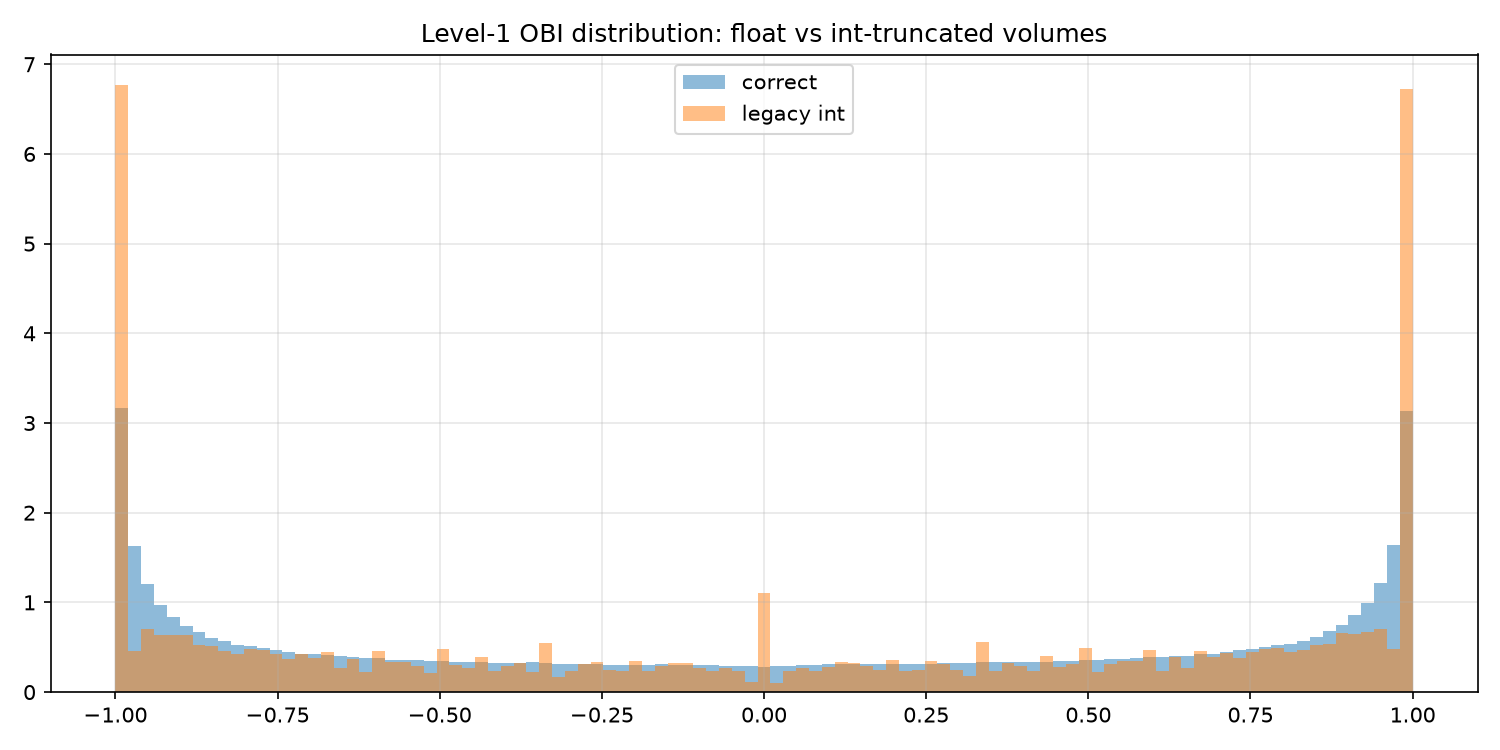
\includegraphics[width=0.8\textwidth]{obi_distribution.png}
\caption{Distribuzione dell'OBI di livello 1 con volumi corretti (\emph{correct}) e troncati
(\emph{legacy int}). La forma a U è reale, ma il troncamento raddoppia il picco a $\pm1$ e crea
masse spurie in $0$ e in valori razionali semplici.}
\label{fig:obi-dist}
\end{figure}

\begin{figure}[H]
\centering
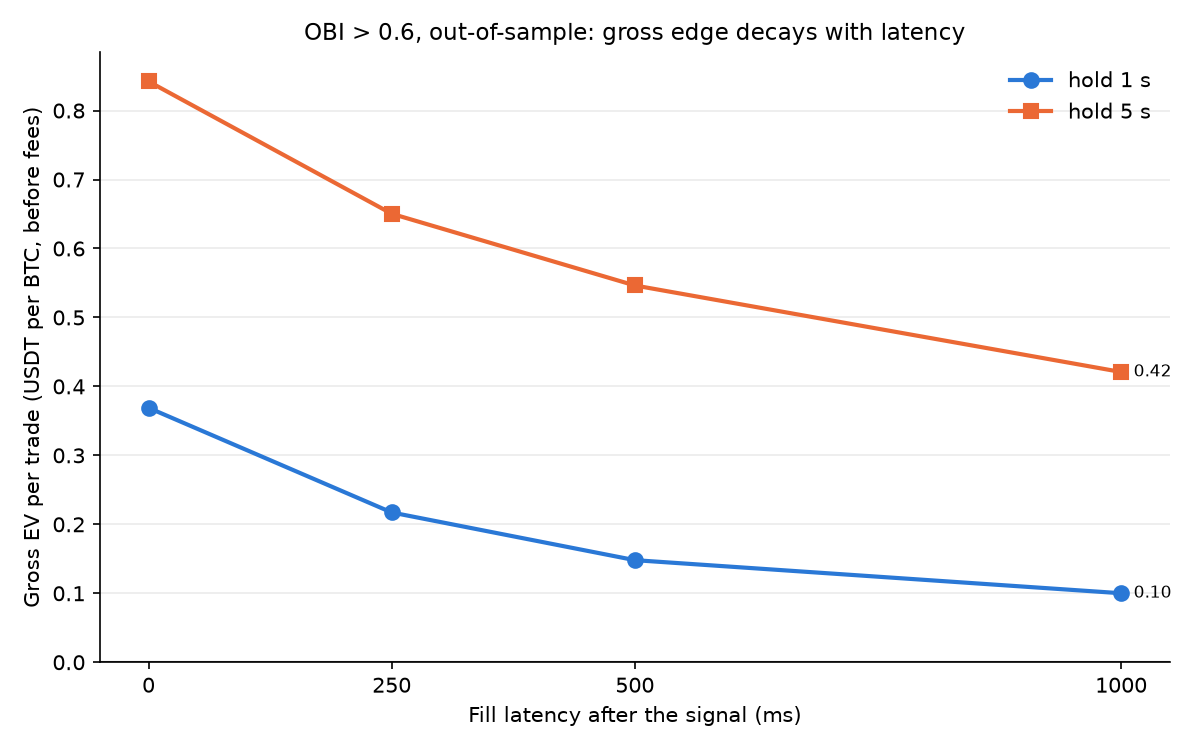
\includegraphics[width=0.7\textwidth]{latency_decay.png}
\caption{EV lordo in funzione della latenza di esecuzione (0, 250, 500, 1000\,ms) per orizzonti
di 1 e 5\,s; OBI $\theta=0.6$, out-of-sample. Stessi dati della Tabella~\ref{tab:latenza}.}
\label{fig:latency-decay}
\end{figure}

\section{Metriche}
\label{app:metriche}

Siano $x_j$ e $g_j$ il PnL netto e lordo degli $N$ trade inclusi, $\bar x$ la media e
$\hat\sigma$ la deviazione standard campionaria. Uso win rate $=\frac1N\sum_j
\mathbf{1}\{x_j>0\}$, $\EV_{\mathrm{lordo}} = \frac1N \sum_j g_j$, $\EV_{\mathrm{netto}} = \bar x$,
\begin{gather}
  t = \frac{\bar x}{\hat\sigma/\sqrt{N}}, \qquad
  \mathrm{SR}_{\mathrm{ann}} = \frac{\overline{R}_{\mathrm{giorno}}}{\hat\sigma_{\mathrm{giorno}}}\sqrt{365}, \\
  \mathrm{MDD} = \max_{u} \Big( \max_{v\le u} E_v - E_u \Big),\quad E_u = \textstyle\sum_{j\le u} x_j,
\end{gather}
con $R_{\mathrm{giorno}}$ il PnL netto per giorno UTC di uscita. Un $|t|\gtrsim 2$ corrisponde a
circa il 5\% solo se i trade sono indipendenti, cosa che qui non è vera. Nella
commissione di pareggio~\eqref{eq:breakeven} ricavo il prezzo medio di esecuzione $P$ dagli
stessi risultati come $(\EV_{\mathrm{lordo}} - \EV_{\mathrm{netto}})/(2f)$: circa
19\,500\usdt{} in-sample e 21\,050\usdt{} out-of-sample.

\section{Tutte le assunzioni}
\label{app:assunzioni}

\begin{enumerate}[label=\textbf{A\arabic*.}, leftmargin=*]
  \item \emph{Solo taker}: compro all'ask e vendo al bid; niente ordini limite né fill passivi.
  \item \emph{Latenza}: fill al primo snapshot con $t_j \ge t_k + L$, di default $L = 250$\,ms.
  \item \emph{Prezzo di fill}: il touch dello snapshot di fill, più/meno $\sigma$ (0 nei
        risultati riportati).
  \item \emph{Commissioni}: per lato sul nozionale. Riprezzo gli stessi trade a più livelli di
        commissione (0, 2 e 4\bp{} per l'OBI, 0 e 4\bp{} per il WOBI), perché la selezione dei
        trade non dipende dalle commissioni.
  \item \emph{Una posizione alla volta}, selezione greedy, rientro possibile sullo snapshot di
        uscita.
  \item \emph{Orizzonti in tempo reale}: orizzonti e time-stop in ms dal fill.
  \item \emph{Gap}: trade attraversati da un intervallo $>2\,000$\,ms esclusi dalle statistiche.
  \item \emph{Fine dati}: bracket chiuso sull'ultimo snapshot; a orizzonte fisso trade scartato.
  \item \emph{Size}: PnL per 1\,BTC, nessun impatto di mercato.
  \item \emph{Nessuna coda}: non stimo posizione in coda né probabilità di fill.
  \item \emph{Bracket su dati discreti}: take-profit e stop-loss sono controllati sul prezzo di
        uscita (touch $\mp\sigma$) di ogni snapshot; ciò che succede tra due snapshot non lo
        vedo.
  \item \emph{Validazione}: split cronologico 70/30; i segnali dipendono solo dallo snapshot
        corrente e le soglie non sono stimate dai dati, quindi non c'è leakage.
  \item \emph{Statistica}: t-stat e intervalli di confidenza assumono trade indipendenti.
  \item \emph{Sharpe}: annualizzato con $\sqrt{365}$ dal PnL giornaliero, solo indicativo.
\end{enumerate}

% ---------------------------------------------------------------------------
\begin{thebibliography}{9}

\bibitem{kaggle}
Bitcoin Limit Order Book (LOB) Data (BTCUSDT perpetual, Binance), dataset Kaggle, licenza MIT.
\url{https://www.kaggle.com/datasets/siavashraz/bitcoin-perpetualbtcusdtp-limit-order-book-data}.

\end{thebibliography}

\end{document}
